%****************************************************************
\section{Parameters Screening}\label{sec:sa_parameters_screening}
%****************************************************************

Screening methods are used to rank the importance of the model parameters using a relatively small number of model evaluations \cite{Saltelli2004}.
However, they tend to simply give qualitative measures.
That is, meaningful information resides in the rank itself but not in the exact importance of the parameters with respect to the output. 
Screening is particularly valuable in the early phase of a SA to identify the noninfluential parameters of a model,
which then could be safely excluded from further detailed analysis. 
This step is important to reduce the size of the problem especially if more expensive methods are to be applied at the subsequent steps. 
In this work, attention was paid to a particular screening method proposed by Morris \cite{Morris1991} with an extension proposed by Campolongo et al. \cite{Campolongo2011}.

\subsection{Elementary Effects and One-at-a-Time Design}\label{sub:sa_ee_oat}

Consider a model with $D$ parameters, where $\mathbf{x} = (x_1, x_2, \dots,x_D)$ is a vector of parameter value evaluated at point $\mathbf{x}$.
The elementary effect of the $d$-th parameter is defined as
\marginpar{elementary effect}
\begin{equation}
EE_d = \frac{y(x_1, \dots, x_d+\Delta,\dots,x_D) - y(x_1, \dots, x_d,\dots,x_D)}{\Delta}
\end{equation}
where $\Delta$, the grid jump, is chosen such that $\mathbf{x} + \Delta$ is still in the specified domain of the parameter space, i.e., $[0,1]^D$; 
$\Delta$ is a value in $\{\frac{1}{p-1}, \dots, 1 - \frac{1}{p-1}\}$, 
where $p$ is the number of (discretization) levels that partition the model parameter space into a uniform grid of points at which the model can be evaluated. 
For a given $p$, the grid constructs a finite distribution of $p^{D-1}[p - \Delta(p-1)]$ elementary effects for each input parameter.

The elementary effect distributions for each of the parameters, evaluated across discretized input parameter space, 
\marginpar{\gls{oat} experimental design}
provide useful information on the importance of a parameter on the output.
Unfortunately, an exhaustive evaluation of all elementary effects for a given discretization levels suffers from a curse of dimensionality especially for numerous parameters and/or for reasonably fine discretization level\footnote{for $p = 8$ and $D = 20$ the total number of evaluations for exhaustive computation of all $EE$s is $\approx 6 \times 10^{17}$ for each parameter}.
Consequently, a class of design of experiment that only change one parameter at a time (\gls{oat}) are devised to estimate the statistics of the distributions.
  
The key idea behind the original Morris method is in initiating the model evaluations from various \textit{nominal} points, $\mathbf{x}$,
\marginpar{trajectory OAT design}
randomly selected over the grid and then gradually advancing one grid jump, perturbing one parameter at a time.
The order of perturbation (i.e., which dimension to perturb first) and the direction of the perturbation (i.e., whether it is added or subtracted) are also randomized between replications.
As such, different replication generates different starting nominal point as well as different order and sign (but with with the same size) of perturbation.
The \gls{oat} computer experimental design complemented with this requirement is known as the trajectory design \cite{Ruano2012}.
Fig.~\ref{fig:ch3_plot_oat_illustration_1} illustrates a trajectory design in two-dimensional input parameter space discretized in $6$ levels with 4 design replications.
\normdoublefigure[pos=tbhp,
                  mainlabel={fig:ch3_plot_oat_illustration},
                  maincaption={Illustration of One-at-a-Time (OAT) design constructed using trajectory scheme (left) and radial scheme (right) each with 4 replications. The trajectory design is discretized in 6 levels, while the number of levels is irrelevant for radial design. Filled circles are the nominal (for the trajectory) or base(for the radial) points and crosses are the perturbed levels.},%
									mainshortcaption={Illustration of One-at-a-Time (OAT) design using trajectory and radial schemes.},
                  leftopt={width=0.45\textwidth},
                  leftlabel={fig:ch3_plot_oat_illustration_1},
                  leftcaption={Trajectory scheme},
                  %leftshortcaption={},%
                  rightopt={width=0.45\textwidth},
                  rightlabel={fig:ch3_plot_oat_illustration_2},
                  rightcaption={Radial scheme},
                  %rightshortcaption={},
                  %spacing={\hfill}
                 ]
{../figures/chapter3/figures/plotOATIllustration_1}
{../figures/chapter3/figures/plotOATIllustration_2}

To remove the requirement to specify a method-specific parameter $p$ (the number of levels),
\marginpar{radial OAT design}
Campolongo et al.\cite{Campolongo2011} proposed to use a radial scheme coupled with Sobol' quasirandom sequence.
In a single replication of this particular OAT design, 
each parameter is perturbed relative to a \textit{base/nominal} point 
which is not required to be located in a predetermined grid.
The size and sign of the perturbation is also allowed to vary from parameter to parameter in different replication.
As such, radial design implicitly incorporates several additional possible sources of variation in the method 
that can potentially bias the estimation of elementary effects.
Because the size of parameter perturbations varies, the definition of the elementary effects is slightly changed to,
\marginpar{elementary effect for radial design}
\begin{equation}
EE_d = \frac{y(x_1, \dots, x_d+\Delta x_d,\dots,x_D) - y(x_1, \dots, x_d,\dots,x_D)}{\Delta x_d}
\end{equation}
where now each parameter at each design replication has its corresponding perturbation size $\Delta x_d \in [-1,1]$ such that $x_d + \Delta x_d \in [0,1]$.

An illustration of a radial design in two-dimensional input space with $4$ base points is shown in Fig.~\ref{fig:ch3_plot_oat_illustration_2}.
 
%-------------------------------------------------------------------------------------------------
\subsection{Statistics of Elementary Effects and Sensitivity Measures}\label{sub:sa_ee_statistics}
%-------------------------------------------------------------------------------------------------

% Mean of the elementary effects
Consider now that an $N_R$ number of elementary effects associated with the $d$-th parameter have been sampled from the finite distribution of $EE_d$,
using a \gls{oat} design with $N_R$ replications.
The statistical summary of sampled $EE_d$ based on a given number of OAT design replications generated using either the trajectory or the radial design can be calculated.
The first is the arithmetic mean defined as,
\marginpar{the mean of the (sampled) elementary effects}
\begin{equation}
	\mu_d = \frac{1}{N_R} \sum_{r = 1}^{N_R} EE^r_d
	\label{eq:sa_morris_mu}
\end{equation} 
where $EE^r_d$ is the elementary effect of the $d$-th parameter of the $r$-th replication.
The mean gives the global influence of the $d$-th parameter on the chosen output $f$.

% Standard deviation of the elementary effects
The second statistical summary of interest is the standard deviation of the (sampled) elementary effects for input parameter $x_d$,
\marginpar{the standard deviation of the (sampled) elementary effects}
\begin{equation}
	\sigma_d = \sqrt{\frac{1}{N_R} \sum_{r = 1}^{N_R} (EE^r_d - \mu_d)^2}
	\label{eq:sa_morris_sd}
\end{equation} 
The standard deviation gives an indication of the presence of nonlinearity and/or interactions between the $d$-th input parameter and the others.

% Mean of absolute values of the elementary effects
In cases where $f$ is a non-monotonic function,
the sign of $EE_d$ may change according to the change of the output,
and cancellation effects on the estimation of $\mu_d$ might occur 
(as can be the case for a non-monotonic function).
To circumvent this issue,
Campolongo et al (\cite{Campolongo2011}) proposed to take the absolute values of the sampled elementary effects.
It is defined as,
\marginpar{the mean of the (sampled) absolute elementary effects}
\begin{equation}
	\mu^*_d = \frac{1}{N_R} \sum_{r = 1}^{N_R} |EE^r_d|
	\label{eq:sa_morris_mustar}
\end{equation}
Note that although the overall sign of output perturbation is lost by using this measure,
its use is justified if parameters are to be ranked based on a single importance measure.

% Interpretation and importance classification
The aforementioned statistical summaries, when evaluated over a large number of replications $N_R$,
can provide global sensitivity measures of the importance of each input parameter.
\marginpar{input parameter importance classification}
As indicated by Morris \cite{Morris1991}, there are three possible categories of parameter importance based on those statistics:
\begin{enumerate}
	\item Parameters with noninfluential effects, i.e., the parameters that have relatively small values of both $\mu_d$ (or $\mu^*_d$) and $\sigma_d$;
	The parameter has a negligible overall effect on the model output.
	\item Parameters with linear and/or additive effects, i.e., the parameters that have relatively large value of $\mu_d$ (or $\mu^*_d$) and relatively small value of $\sigma_d$.
	The small value of $\sigma_d$ and the large value of $\mu_d$ (or $\mu^*_d$) indicate that the variation of elementary effects across replications is small while the magnitude of the effect itself is consistently large for the perturbations in the parameter space.
	\item Parameters with nonlinear and/or interaction effects, i.e., the parameters that have a relatively small value of $\mu_d$ (or $\mu^*_d$) and a relatively large value of $\sigma_d$.
	Opposite to the previous case, a small value of $\mu_d$ (or $\mu^*_d$) indicates that the aggregate effect of perturbation is relatively small (or in the case of $\mu_d$, can be close to zero) while a large value of $\sigma_d$ indicates that the variation of the effect is large; the effect can be large or negligibly small depending on the values of the other parameters at which the model is evaluated.
	Such large variation is a symptom of nonlinear effects and/or parameter interaction.
\end{enumerate}

% Classification and qualitative measure
Such classification makes parameter importance ranking and, in turn, screening of noninfluential parameters possible.
However, the procedure is done rather qualitatively, and this is illustrated in Fig.~\ref{fig:illustration_morris_result}, 
which depicts a typical parameter classification derived from visual inspection of the elementary effects statistics on the $\sigma$ vs. $\mu^*$ plane.
The notions of influential and noninfluential parameters are based on the relative locations of those statistics in the plane.
Typically, the noninfluential ones are clustered closer to the origin (relative to the more influential ones) with a pronounced boundary such as the one depicted in Fig.~\ref{fig:illustration_morris_result}. 
Admittedly, if these statistics are spread somewhat uniformly across the plane, 
the distinction would be more ambiguous and problematic\footnote{In such a case, a more advanced classification such as the ones based on clustering techniques might be helpful to identify a finer structure of the parameters importance.}.
Furthermore, for a parameter with a large value of both $\mu^*$ and $\sigma$,
the method cannot distinguish between nonlinearity effect from parameter interaction effect on the output.

\begin{figure}[bth]
	\centering
	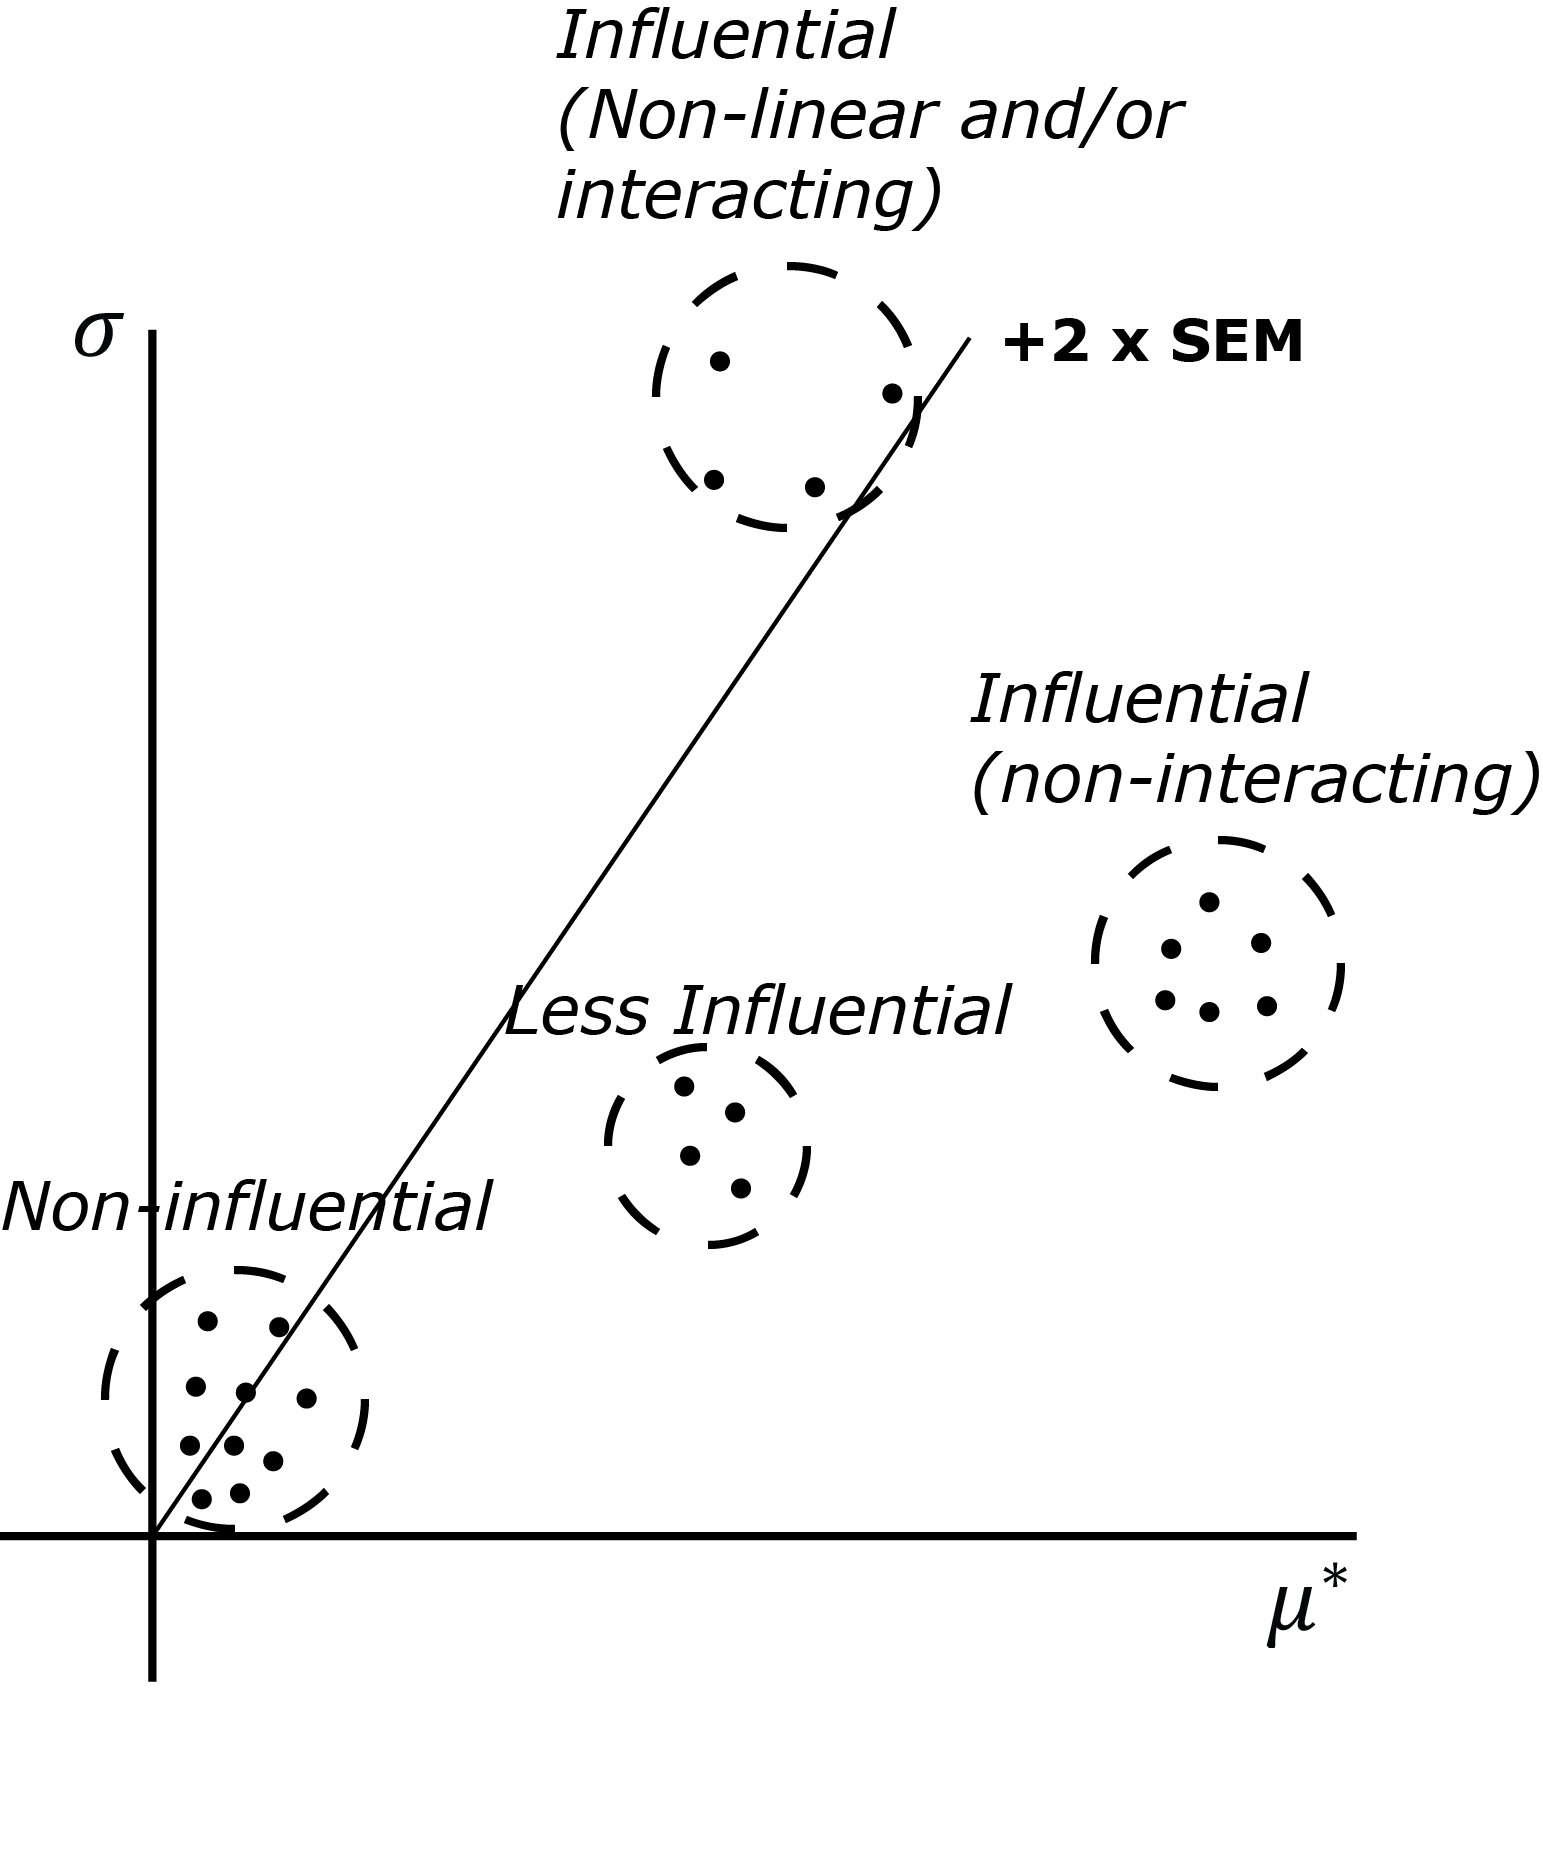
\includegraphics[scale=0.90]{../figures/illustrateMorrisResult/illustrateMorrisResult.png}
	\caption[Illustration of a typical parameter importance classification based on Morris screening method]{Illustration of a typical parameter importance classification obtained from the Morris screening method. The importance of each parameter relative to the other ones is defined with respect to its location on the $\sigma - \mu^*$ plane. Each dot represents a parameter, and the line corresponds to twice the standard error of the mean (SEM) indicating the relative magnitude of the standard deviation to the mean.}\label{fig:illustration_morris_result}
\end{figure}
